\chapter{Первая программа}

\subsubsection{Коды программы}

\begin{center}
    \captionsetup{justification=raggedright,singlelinecheck=off}
    \begin{lstlisting}[label=lst:CIO1,caption=Один поток]
#include <stdio.h>
#include <fcntl.h>

#define RESET   "\033[0m"
#define RED     "\033[1;31m"
#define BLUE    "\033[1;34m"

int main(void)
{
    int fd = open("alphabet.txt", O_RDONLY);
    
    FILE *fs1 = fdopen(fd, "r");
    char buff1[20];
    setvbuf(fs1, buff1, _IOFBF, 20);
    
    FILE *fs2 = fdopen(fd, "r");
    char buff2[20];
    setvbuf(fs2, buff2, _IOFBF, 20);
    
    int flag1 = 1, flag2 = 2;
    
    while (flag1 == 1 || flag2 == 1)
    {
        char c;
        flag1 = fscanf(fs1, "%c", &c);

        if (flag1 == 1) 
        {
            fprintf(stdout, RED "%c" RESET, c);
        }

        flag2 = fscanf(fs2, "%c", &c);

        if (flag2 == 1)
        { 
            fprintf(stdout, BLUE "%c" RESET, c); 
        }
    }

    fprintf(stdout, "\n");
    return 0;
}
\end{lstlisting}
\end{center}

\begin{center}
    \captionsetup{justification=raggedright,singlelinecheck=off}
    \begin{lstlisting}[label=lst:CIO2,caption=Два потока]
#include <stdio.h>
#include <fcntl.h>
#include <pthread.h>

#define RESET   "\033[0m"
#define RED     "\033[1;31m"
#define BLUE    "\033[1;34m"

typedef struct args
{
    FILE *fs;
    char *color;
} arg_struct;

void *print_letter(void *arg) 
{
    arg_struct *now_arg = (arg_struct *) arg;
    FILE *fs = now_arg->fs;

    int flag = 1;
    char c;

    while (flag == 1) 
    {
        flag = fscanf(fs, "%c", &c);

        if (flag == 1)
        {
            fprintf(stdout, "%s%c" RESET, now_arg->color, c);

            sleep(1);
        }
    }

    return NULL;
}

int main(void)
{
    int fd = open("alphabet.txt", O_RDONLY);
    
    FILE *fs1 = fdopen(fd, "r");
    char buff1[20];
    setvbuf(fs1, buff1, _IOFBF, 20);
    arg_struct arg1 = {.fs = fs1, .color = RED};
    
    FILE *fs2 = fdopen(fd, "r");
    char buff2[20];
    setvbuf(fs2, buff2, _IOFBF, 20);
    arg_struct arg2 = {.fs = fs2, .color = BLUE};
    pthread_t tid;
    pthread_create(&tid, NULL, print_letter, &arg2);

    print_letter(&arg1);

    pthread_join(tid, NULL);
    fprintf(stdout, "\n");

    return 0;
}
\end{lstlisting}
\end{center}

\subsubsection{Результаты выполнения программ}

\begin{figure}[H]
	\begin{center}
		
\includegraphics[scale=0.4]{img/CIO1.png}
	\end{center}
	\captionsetup{justification=centering}
	\caption{Результат работы первой программы: один поток}
	\label{img:CIO1}
\end{figure}

\begin{figure}[H]
	\begin{center}
		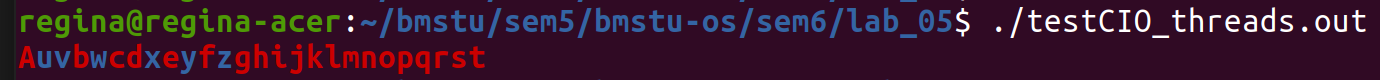
\includegraphics[scale=0.35]{img/CIO2.png}
	\end{center}
	\captionsetup{justification=centering}
	\caption{Результат работы первой программы: два потока}
	\label{img:CIO2}
\end{figure}

\subsubsection{Анализ полученных результатов}

С помощью системного вызова \texttt{open()} создается дескриптор открытого файла \texttt{alphabet.txt} с правами доступа на чтение (\texttt{O\_RDONLY}). Созданному дескриптору соответствует индекс в таблице дескрипторов файлов, открытых процессом, равный 3, так как 0, 1 и 2 заняты \texttt{stdin}, \texttt{stdout} и \texttt{stderr}, и другие файлы процессом не открывались. \texttt{fd[3]} указывает на \texttt{struct file}, которая связана с \texttt{struct inode}, соответствующей файлу \texttt{alphabet.txt}.

С помощью двух вызовов функции \texttt{fdopen()} стандартной библиотеки создаются две структуры \texttt{FILE} --- \texttt{fs1} и \texttt{fs2}, поле \texttt{\_fileno} которых содержит значение 3.

Функция \texttt{setvbuf} устанавливает буферы для каждой из структур \texttt{FILE}, параметрами функции являются указатель на начало, размер (20 байт) и тип буферизации (полная буферизация). Указатель на конец буфера устанавливается через указатель на начало буфера и его размер.

В цикле \texttt{while} реализован поочередный вызов функции \texttt{fscanf()} стандартной библиотеки для \texttt{fs1} и \texttt{fs2}. При первом вызове \texttt{fscanf()} для \texttt{fs1} буфер этой структуры будет заполнен полностью --- в него запишутся 20 символов от 'A' до 't', так как была установлена полная буферизация. В структуре \texttt{struct file} поле \texttt{f\_pos} установится на символ 'u', следующий за символом 't'. Переменная \texttt{c} будет инициализирована символом 'A' и будет выведена на экран. При первом вызове \texttt{fscanf()} для \texttt{fs2} буфер этой структуры будет заполнен символами от 'u' до 'z', так как \texttt{fs1} и \texttt{fs2} ссылаются на один и тот же дескриптор, поле \texttt{f\_pos} которой  указывает на символ 'u'. Этот символ запишется в переменную \texttt{c} и выведется на экран. В следующих вызовах \texttt{fscanf()} переменной \texttt{c} будут поочередно присваиваться символы из каждого буфера и выводиться на экран. Когда один из буферов будет прочитан полностью, на экран будут выводиться символы только из одного буфера, что показано на рисунке \ref{img:CIO1}. Файл был полностью прочитан при первом вызове \texttt{fscanf()} для \texttt{fs2}, поэтому повторных заполнений не будет.

В многопоточной реализации в зависимости от того, какой поток первым вызовет \texttt{fscanf()} возможны различные варианты, один из которых представлен на рисунке \ref{img:CIO2}.

\begin{figure}[H]
	\begin{center}
		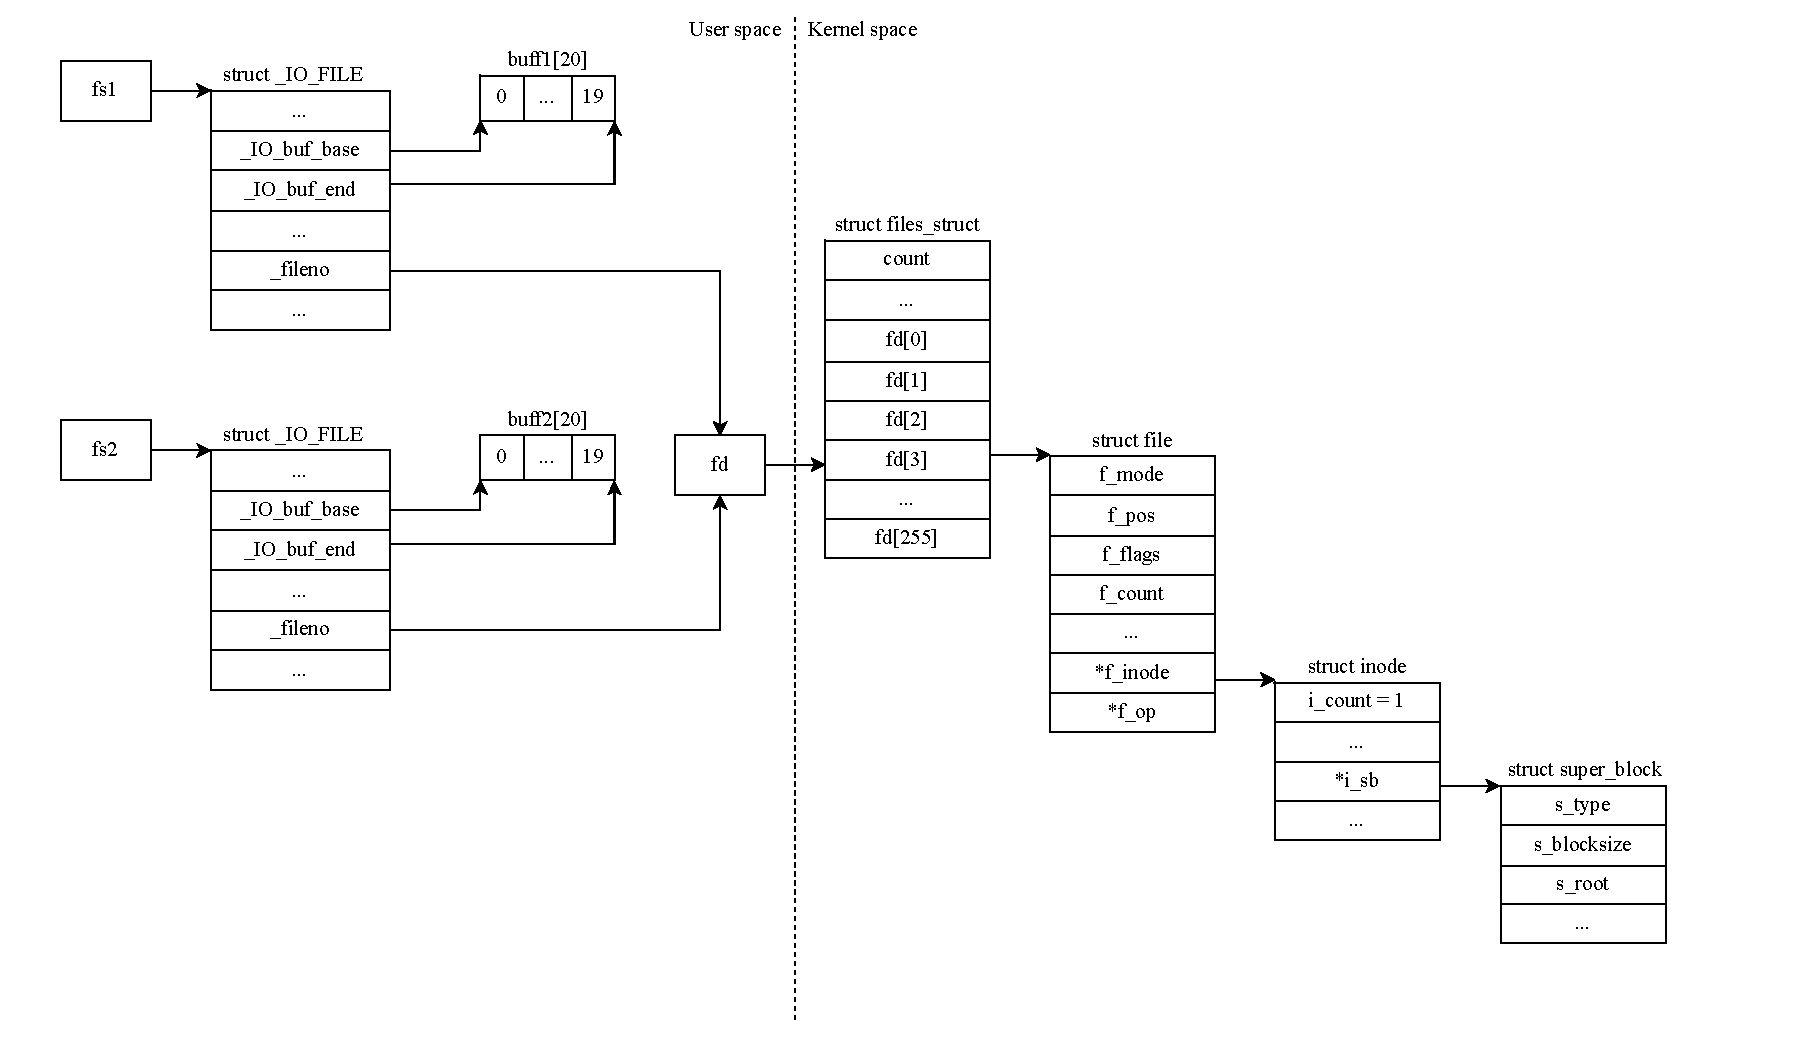
\includegraphics[scale=0.6]{img/CIO.pdf}
	\end{center}
	\captionsetup{justification=centering}
	\caption{Связь между созданными дескрипторами в первой программе}
	\label{img:CIO}
\end{figure}

\chapter{Вторая программа}

\subsubsection{Коды программ}

\begin{center}
    \captionsetup{justification=raggedright,singlelinecheck=off}
    \begin{lstlisting}[label=lst:kernelIO1,caption=Один поток]
#include <fcntl.h>
#include <unistd.h>

#define RESET   "\033[0m"
#define RED     "\033[1;31m"
#define BLUE    "\033[1;34m"

int main(void)
{
    char c;    

    int fd1 = open("alphabet.txt", O_RDONLY);
    int fd2 = open("alphabet.txt", O_RDONLY);

    int flag1 = 1, flag2 = 2;

    while (flag1 == 1 || flag2 == 1)
    {
        flag1 = read(fd1, &c, 1);

        if (flag1 == 1)
        {
            printf(RED "%c" RESET, c);
        }

        flag2 = read(fd2, &c, 1);

        if (flag2 == 1)
        {
            printf(BLUE "%c" RESET, c);
        }
    }

    printf("\n");
    return 0;
}
\end{lstlisting}
\end{center}

\begin{center}
    \captionsetup{justification=raggedright,singlelinecheck=off}
    \begin{lstlisting}[label=lst:kernelIO2,caption=Два потока]
#include <fcntl.h>
#include <unistd.h>
#include <pthread.h>

#define RESET   "\033[0m"
#define RED     "\033[1;31m"
#define BLUE    "\033[1;34m"

typedef struct args
{
    int fd;
    char *color;
} arg_struct;

pthread_mutex_t mutex;

void *print_letter(void *arg) 
{
    pthread_mutex_lock(&mutex);
    arg_struct *now_arg = (arg_struct *) arg;
    int fd = now_arg->fd;

    int flag = 1;
    char c;

    while (flag == 1) 
    {
        flag = read(fd, &c, 1);

        if (flag == 1)
        {
            printf("%s%c" RESET, now_arg->color, c);
        }
    }

    pthread_mutex_unlock(&mutex);

    return NULL;
}

int main(void)
{
    int fd1 = open("alphabet.txt", O_RDONLY);
    arg_struct arg1 = {.fd = fd1, .color = RED};

    int fd2 = open("alphabet.txt", O_RDONLY);
    arg_struct arg2 = {.fd = fd2, .color = BLUE};
    pthread_t tid;
    pthread_create(&tid, NULL, print_letter, &arg2);

    print_letter(&arg1);

    pthread_join(tid, NULL);

    printf("\n");
    return 0;
}
\end{lstlisting}
\end{center}

\subsubsection{Результаты выполнения программ}

\begin{figure}[H]
	\begin{center}
		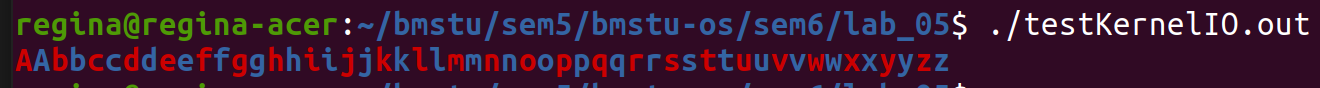
\includegraphics[scale=0.35]{img/kernelIO1.png}
	\end{center}
	\captionsetup{justification=centering}
	\caption{Результат работы второй программы: один поток}
	\label{img:kernelIO1}
\end{figure}

\begin{figure}[H]
	\begin{center}
		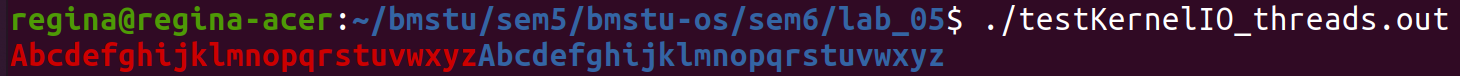
\includegraphics[scale=0.3]{img/kernelIO2.png}
	\end{center}
	\captionsetup{justification=centering}
	\caption{Результат работы второй программы: два потока}
	\label{img:kernelIO2}
\end{figure}

\subsubsection{Анализ полученных результатов}

Два системных вызова \texttt{open()} открывают файл \texttt{alphabet.txt} для чтения (\texttt{O\_RDONLY}) и создают два дескриптора открытого файла, которым присваиваются значения 3 и 4. При этом создаются две структуры \texttt{struct file}, которые ссылаются на одну и ту же структуру \texttt{struct inode}. Поля \texttt{f\_pos} двух структур \texttt{struct file} изменяются независимо друг от друга, поэтому для каждого файлового дескриптора происходит полное чтение файла, и каждый символ (от 'A' до 'z') будет выведен два раза, что показано на рисунке \ref{img:kernelIO1}.

При многопоточной реализации символы дублируются, но порядок их вывода хаотичен. Добавление в программу мьютекса \texttt{pthread\_mutex\_t mutex} приводит к тому, что алфавит выводится полностью два раза, как показано на рисунке \ref{img:kernelIO2}.

\begin{figure}[H]
	\begin{center}
		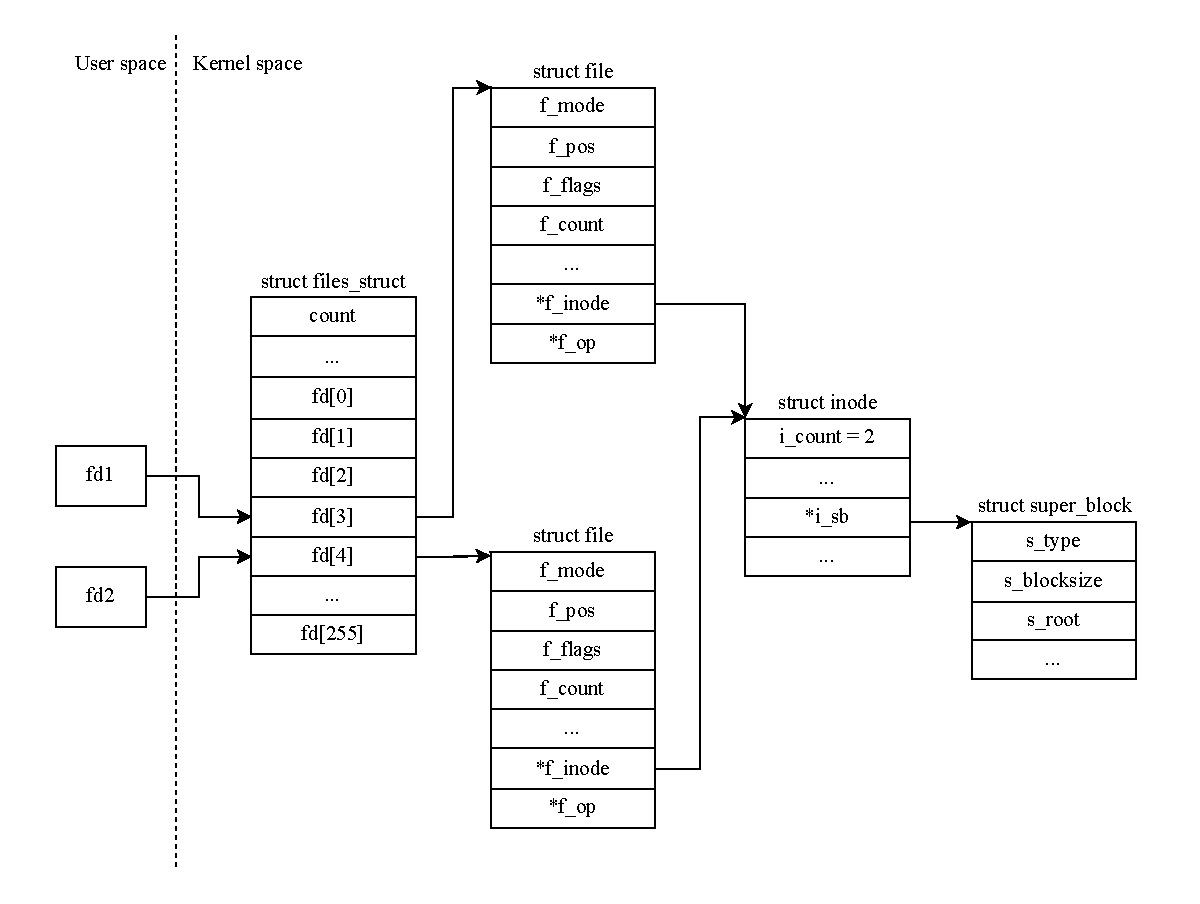
\includegraphics[scale=0.8]{img/kernelIO.pdf}
	\end{center}
	\captionsetup{justification=centering}
	\caption{Связь между созданными дескрипторами во второй программе}
	\label{img:kernelIO}
\end{figure}

\chapter{Третья программа}

\subsubsection{Коды программ}

\begin{center}
    \captionsetup{justification=raggedright,singlelinecheck=off}
    \begin{lstlisting}[label=lst:task31,caption=Один поток]
#include <stdio.h>
#include <sys/stat.h>

void print_file_info(FILE *fs) 
{
    struct stat buff;
    stat("results.txt", &buff);
    printf("inode: %ld\n", buff.st_ino);
    printf("Размер в байтах: %ld\n", buff.st_size);
    printf("Текущая позиция: %ld\n\n", ftell(fs));
}

int main(void)
{
    char c;    

    FILE* fs1 = fopen("results.txt", "w");
    print_file_info(fs1);

    FILE* fs2 = fopen("results.txt", "w");
    print_file_info(fs2);

    for (char c = 'a'; c <= 'z'; c++) 
    {
        if (c % 2) 
        {
            fprintf(fs1, "%c", c);
        } 
        else 
        {
            fprintf(fs2, "%c", c);
        }
    }

    print_file_info(fs1);
    fclose(fs1);
    print_file_info(fs1);

    print_file_info(fs2);    
    fclose(fs2);
    print_file_info(fs2); 

    return 0;
}
\end{lstlisting}
\end{center}

\begin{center}
    \captionsetup{justification=raggedright,singlelinecheck=off}
    \begin{lstlisting}[label=lst:task32,caption=Два потока]
#include <stdio.h>
#include <pthread.h>

void *print_letter(void *arg) 
{
    FILE* fd = fopen("results.txt", "a");
    char *c = (char *) arg;

    while (*c <= 'z')
    {
        fprintf(fd, "%c", *c);
        (*c) += 2;
    }

    fclose(fd);

    return NULL;
}

int main(void)
{
    pthread_t tid;
    char c2 = 'b', c1 = 'a';
    pthread_create(&tid, NULL, print_letter, &c2);

    print_letter(&c1);
    pthread_join(tid, NULL);

    return 0;
}
\end{lstlisting}
\end{center}

\subsubsection{Результаты выполнения программ}

\begin{figure}[H]
	\begin{center}
		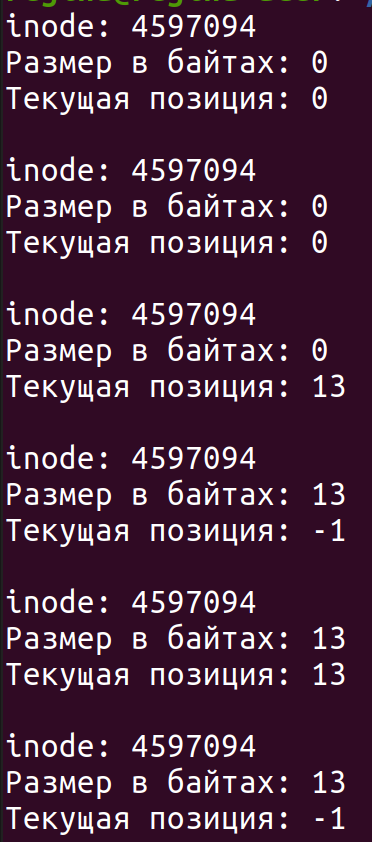
\includegraphics[scale=0.3]{img/info.png}
	\end{center}
	\captionsetup{justification=centering}
	\caption{Информация о файле}
	\label{img:info}
\end{figure}

\begin{figure}[H]
	\begin{center}
		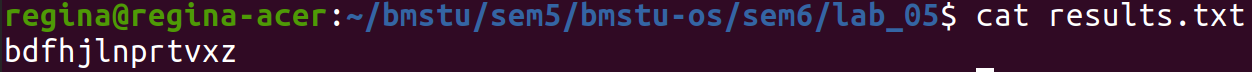
\includegraphics[scale=0.3]{img/task31.png}
	\end{center}
	\captionsetup{justification=centering}
	\caption{Результат работы третьей программы: один поток, последний вызов fclose() для fs2}
	\label{img:task31}
\end{figure}

\begin{figure}[H]
	\begin{center}
		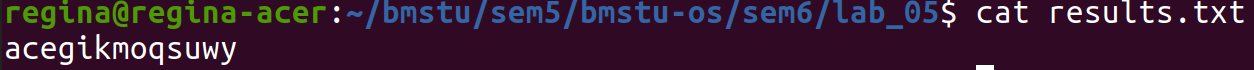
\includegraphics[scale=0.3]{img/task312.png}
	\end{center}
	\captionsetup{justification=centering}
	\caption{Результат работы третьей программы: один поток, последний вызов fclose() для fs1}
	\label{img:task312}
\end{figure}

\begin{figure}[H]
	\begin{center}
		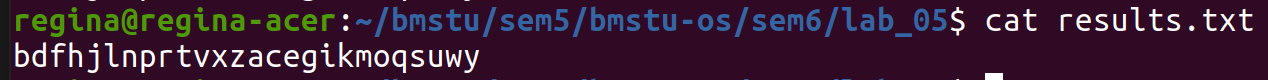
\includegraphics[scale=0.3]{img/task32.png}
	\end{center}
	\captionsetup{justification=centering}
	\caption{Результат работы третьей программы: два потока}
	\label{img:task32}
\end{figure}

\subsubsection{Анализ полученных результатов}

Два вызова функции \texttt{fopen()} стандартной библиотеки открывают файл \texttt{results.txt} для записи (\texttt{"w"}) и создают два дескриптора открытого файла, которым присваиваются значения 3 и 4. При этом создаются две структуры \texttt{struct file}, которые ссылаются на одну и ту же структуру \texttt{struct inode}. Так как по умолчанию используется полная буферизация, запись в файл происходит либо при полном заполнении буфера, либо при вызове \texttt{fflush()} или \texttt{fclose()}. 

В реализации используется вызов \texttt{fclose()}. В цикле \texttt{for} с помощью поочередной передачи функции \texttt{fprintf} дескрипторов \texttt{fs1} и \texttt{fs2} в файл записываются буквы латинского алфавита (от 'a' до 'z') до вызовов \texttt{fclose()}. При вызове \texttt{fclose(fs1)} в файл записываются буквы, стоящие на нечетных позициях в порядке алфавита. При вызове \texttt{fclose(fs2)} запись в файл происходит с начала файла, и записанные ранее символы перезапишутся буквами, стоящими на четных позициях в порядке алфавита, так как поле \texttt{f\_pos} соответствующей структуры \texttt{struct file} не менялось. 

Так, если первым идет вызов \texttt{fclose(fs1)}, а затем --- \texttt{fclose(fs2)}, в файл запишутся буквы, стоящие на четных позициях в порядке алфавита, как показано на рисунке \ref{img:task31}. В обратном порядке --- буквы, стоящие на нечетных позициях в порядке алфавита, что показано на рисунке \ref{img:task312}.

В многопоточной реализации аргумент функции \texttt{fopen()} \texttt{mode} равен \texttt{"a"}, поэтому каждая запись будет производиться в конец файла. Буквы алфавита перезаписываться не будут, что представлено на рисунке \ref{img:task32}.

\begin{figure}[H]
	\begin{center}
		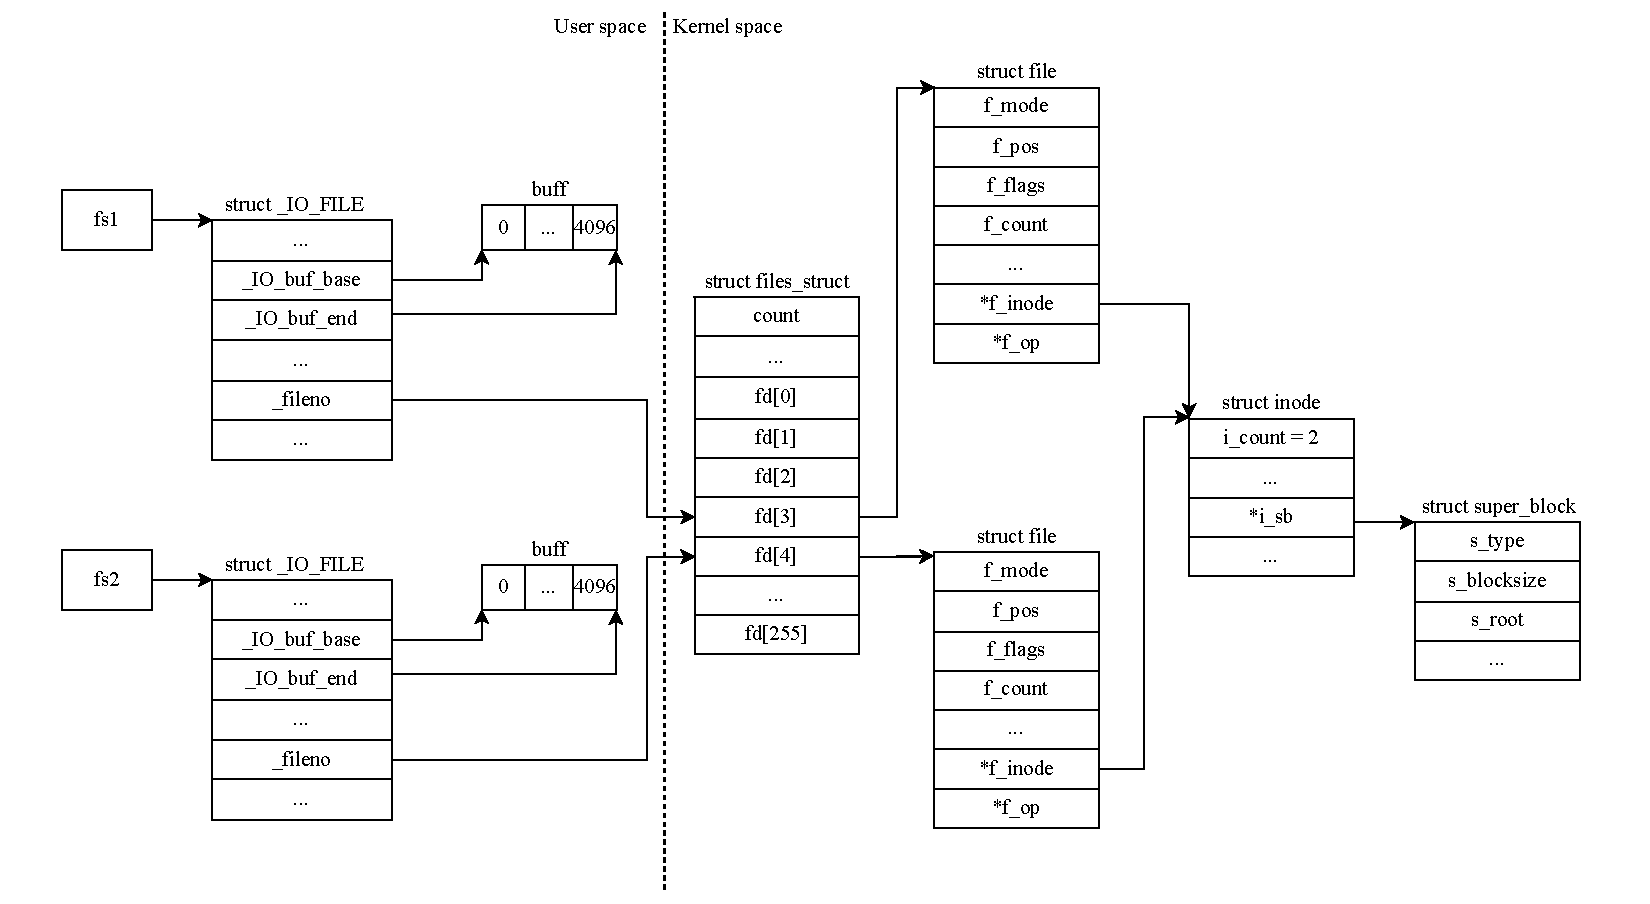
\includegraphics[scale=0.5]{img/task3.pdf}
	\end{center}
	\captionsetup{justification=centering}
	\caption{Связь между созданными дескрипторами в третьей программе}
	\label{img:task3}
\end{figure}

\chapter{Структура FILE}

\begin{center}
    \captionsetup{justification=raggedright,singlelinecheck=off}
    \begin{lstlisting}[label=lst:FILE,caption=Описание структуры FILE в файле /usr/include/x86\_64-linux-gnu/bits/types/FILE.h]
typedef struct _IO_FILE FILE;
\end{lstlisting}
\end{center}

\begin{center}
    \captionsetup{justification=raggedright,singlelinecheck=off}
    \begin{lstlisting}[label=lst:IO\_FILE,caption=Описание структуры \_IO\_FILE в файле /usr/include/x86\_64-linux-gnu/bits/struct\_FILE.h]
struct _IO_FILE
{
  int _flags;		/* High-order word is _IO_MAGIC; rest is flags. */

  /* The following pointers correspond to the C++ streambuf protocol. */
  char *_IO_read_ptr;	/* Current read pointer */
  char *_IO_read_end;	/* End of get area. */
  char *_IO_read_base;	/* Start of putback+get area. */
  char *_IO_write_base;	/* Start of put area. */
  char *_IO_write_ptr;	/* Current put pointer. */
  char *_IO_write_end;	/* End of put area. */
  char *_IO_buf_base;	/* Start of reserve area. */
  char *_IO_buf_end;	/* End of reserve area. */

  /* The following fields are used to support backing up and undo. */
  char *_IO_save_base; /* Pointer to start of non-current get area. */
  char *_IO_backup_base;  /* Pointer to first valid character of backup area */
  char *_IO_save_end; /* Pointer to end of non-current get area. */

  struct _IO_marker *_markers;

  struct _IO_FILE *_chain;

  int _fileno;
  int _flags2;
  __off_t _old_offset; /* This used to be _offset but it's too small.  */

  /* 1+column number of pbase(); 0 is unknown. */
  unsigned short _cur_column;
  signed char _vtable_offset;
  char _shortbuf[1];

  _IO_lock_t *_lock;
#ifdef _IO_USE_OLD_IO_FILE
};

struct _IO_FILE_complete
{
  struct _IO_FILE _file;
#endif
  __off64_t _offset;
  /* Wide character stream stuff.  */
  struct _IO_codecvt *_codecvt;
  struct _IO_wide_data *_wide_data;
  struct _IO_FILE *_freeres_list;
  void *_freeres_buf;
  size_t __pad5;
  int _mode;
  /* Make sure we don't get into trouble again.  */
  char _unused2[15 * sizeof (int) - 4 * sizeof (void *) - sizeof (size_t)];
};
\end{lstlisting}
\end{center}

\chapter{Вывод}

При работе с буферизованным и не буферизованным вводом-выводом возникает ряд следующих проблем.

В первой программе появляется проблема буферизации: символы из файла выводятся не в том порядке, в котором они записаны в файле в связи с включением полной буферизации.

Во второй программе чтение файла и вывод символов производятся два раза, так как два файловых дескриптора связаны с одной структурой \texttt{struct inode}. Добавление мьютекса приводит к созданию разделяемой области памяти.

В третьей программе также возникает проблема буферизации, при этом символы в файле перезаписываются, то есть, происходит потеря информации. Открытие файла в режиме добавления приводит к тому, что запись в файл производится в конец, и потери данных не происходит.

